\documentclass[a4paper,11pt]{article}
\usepackage[utf8]{inputenc}
\usepackage[T1]{fontenc}
\usepackage{amsmath,amssymb}
\usepackage[a4paper,left=2cm,right=2cm,top=3.6cm,bottom=2.3cm,headheight=1.1cm,headsep=0.6cm,footskip=1cm]{geometry}
\usepackage{xcolor}
\usepackage{tikz}
\usetikzlibrary{calc,arrows.meta}
\usepackage{fancyhdr}
\usepackage{lastpage}
\usepackage{tabularx}
\usepackage{array}
\usepackage[most]{tcolorbox}
\usepackage{enumitem}
\usepackage{needspace}

\definecolor{navy}{HTML}{1F3A5F}
\definecolor{teal}{HTML}{0F8B7D}
\definecolor{softbg}{HTML}{F4F7FA}
\definecolor{brick}{HTML}{B03A2E}
\definecolor{amber}{HTML}{D9822B}
\newcommand{\dis}{\displaystyle}

\setlength{\parindent}{0pt}
\renewcommand{\arraystretch}{1.35}

% ---------- header berwarna navy ----------
\pagestyle{fancy}
\fancyhf{}
\renewcommand{\headrulewidth}{0pt}
\fancyhead[L]{%
  \begin{tikzpicture}[remember picture,overlay]
    \fill[navy] ([yshift=-1.2cm]current page.north west) rectangle ([yshift=-3.15cm]current page.north east);
    \fill[teal] ([yshift=-3.15cm]current page.north west) rectangle ([yshift=-3.25cm]current page.north east);
  \end{tikzpicture}%
  \color{white}\bfseries\large Latihan Soal Peluang}
\fancyhead[R]{\color{white}\small Diunduh dari website \textbf{Math1729}\ \,|\,\ 4 Oktober 2026}
\fancyfoot[L]{\small\color{navy}Math1729 --- Peluang}
\fancyfoot[R]{\small\color{navy}Halaman \thepage\ dari \pageref{LastPage}}

% ---------- komponen ----------
\newcounter{no}
\newcommand{\bagian}[2]{\par\Needspace{12\baselineskip}\vspace{1.0em}\noindent
  \begin{tcolorbox}[colback=navy,colframe=navy,coltext=white,boxrule=0pt,arc=2pt,left=6pt,right=6pt,top=3pt,bottom=3pt]
  \textbf{#1}\hfill{\small #2}\end{tcolorbox}\setcounter{no}{0}\par\vspace{-0.3em}}
\newcommand{\tingkat}[2]{\par\Needspace{7\baselineskip}\vspace{0.6em}\noindent
  {\color{teal}\rule{3pt}{1.1em}}\ {\color{navy}\bfseries #1}\ {\small\color{gray}--- #2}\par\vspace{0.1em}}
\newcommand{\soal}[2]{\par\vspace{0.75em}\stepcounter{no}\noindent
  \begin{minipage}[t]{1.8em}\textbf{\theno.}\end{minipage}%
  \begin{minipage}[t]{\dimexpr\linewidth-1.8em\relax}#1\par\vspace{0.35em}#2\end{minipage}\par}
\newcommand{\poin}[1]{\hfill{\small\color{navy}[#1 poin]}}

% teks di kiri, gambar di kanan (nomor soal tetap di baris pertama)
\newcommand{\gbr}[2]{\noindent\begin{minipage}[t]{0.58\linewidth}#1\end{minipage}\hfill\raisebox{\ht\strutbox}{\begin{minipage}[t]{0.39\linewidth}\vspace{0pt}\centering#2\end{minipage}}}
\tikzset{nd/.style={circle,draw=navy,thick,fill=softbg,inner sep=1.5pt,minimum size=0.55cm,font=\small}}
\tikzset{lf/.style={font=\scriptsize,midway,fill=white,inner sep=1pt}}

\begin{document}
\thispagestyle{fancy}

\begin{center}
  {\color{navy}\fontsize{22}{26}\selectfont\bfseries Latihan Soal Peluang\par}
\end{center}
\vspace{2pt}
\begin{tcolorbox}[colback=softbg,colframe=navy!40,boxrule=0.6pt,arc=3pt,left=8pt,right=8pt,top=5pt,bottom=5pt]
\noindent\textbf{Nama} : \rule{4.6cm}{0.4pt}\hfill\textbf{Kelas} : \rule{2.2cm}{0.4pt}\hfill\textbf{Skor} : \rule{2.2cm}{0.4pt}
\end{tcolorbox}
\vspace{2pt}
\begin{tcolorbox}[colback=white,colframe=teal,boxrule=0.8pt,arc=3pt,left=8pt,right=8pt,top=4pt,bottom=4pt,title={\bfseries Petunjuk Pengerjaan},coltitle=white,fonttitle=\small]
\small
\begin{enumerate}[leftmargin=1.4em,itemsep=1pt,topsep=1pt]
\item Soal terdiri atas \textbf{15 pilihan ganda} (5 mudah, 5 sedang, 5 sulit), \textbf{5 isian singkat}, dan \textbf{3 uraian (essay)}. Alokasi waktu yang disarankan: 90 menit.
\item Skor: pilihan ganda 3 poin, isian singkat 5 poin, uraian 10 poin per soal (total 100 poin). Tidak ada pengurangan skor untuk jawaban salah.
\item Semua koin dan dadu dianggap seimbang, dan pengambilan bola atau kartu dilakukan secara acak, kecuali dinyatakan lain. Gambar tidak selalu digambar sesuai skala.
\item Rumus yang boleh dipakai: $P(A)=\dis\frac{n(A)}{n(S)}$, $P(A\mid B)=\dis\frac{P(A\cap B)}{P(B)}$, $\dbinom nr=\dis\frac{n!}{r!\,(n-r)!}$, dan $F_h=n\cdot P(A)$.
\item Jawaban pecahan dituliskan dalam bentuk paling sederhana. Kalkulator tidak diperkenankan.
\end{enumerate}
\end{tcolorbox}

\bagian{A. Pilihan Ganda}{15 soal $\times$ 3 poin = 45 poin. Pilih satu jawaban yang paling tepat.}

\tingkat{Tingkat Mudah}{soal 1 sampai 5}
\soal{\gbr{Sebuah roda putar dibagi menjadi $10$ sektor sama besar yang diberi nomor $1$ sampai $10$ (lihat gambar). Jika roda diputar dan jarum berhenti secara acak, peluang jarum berhenti pada sektor bernomor prima adalah \dots.}{%
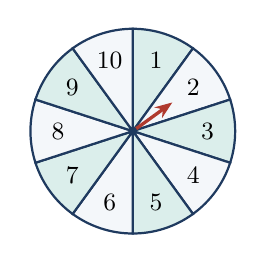
\begin{tikzpicture}
\foreach \i in {1,...,10}{%
  \pgfmathsetmacro{\a}{90-36*(\i-1)}
  \pgfmathsetmacro{\b}{\a-36}
  \pgfmathsetmacro{\m}{\a-18}
  \ifodd\i \def\cc{teal!15}\else\def\cc{softbg}\fi
  \draw[navy,thick,fill=\cc] (0,0)--(\a:1.3) arc (\a:\b:1.3)--cycle;
  \node[font=\small] at (\m:0.95) {\i};}
\draw[brick,very thick,-{Stealth[length=2.2mm]}] (0,0)--(36:0.62);
\fill[navy] (0,0) circle (1.6pt);
\end{tikzpicture}}}{\begin{tabularx}{\linewidth}{@{}*{5}{X}@{}}\textbf{A.}\;$\dis\frac15$ & \textbf{B.}\;$\dis\frac3{10}$ & \textbf{C.}\;$\dis\frac25$ & \textbf{D.}\;$\dis\frac12$ & \textbf{E.}\;$\dis\frac35$\end{tabularx}}
\soal{Dua dadu seimbang dilempar bersamaan. Peluang jumlah kedua mata dadu paling sedikit $9$ adalah \dots.}{\begin{tabularx}{\linewidth}{@{}*{5}{X}@{}}\textbf{A.}\;$\dis\frac5{18}$ & \textbf{B.}\;$\dis\frac13$ & \textbf{C.}\;$\dis\frac5{12}$ & \textbf{D.}\;$\dis\frac12$ & \textbf{E.}\;$\dis\frac7{12}$\end{tabularx}}
\soal{Sebuah kartu diambil acak dari kartu bernomor $1$ sampai $12$. Peluang terambil kartu bernomor kelipatan $3$ atau kelipatan $4$ adalah \dots.}{\begin{tabularx}{\linewidth}{@{}*{5}{X}@{}}\textbf{A.}\;$\dis\frac14$ & \textbf{B.}\;$\dis\frac13$ & \textbf{C.}\;$\dis\frac5{12}$ & \textbf{D.}\;$\dis\frac12$ & \textbf{E.}\;$\dis\frac7{12}$\end{tabularx}}
\soal{\gbr{Sebuah dadu dilempar $50$ kali dan hasilnya dicatat pada tabel. Peluang empiris muncul mata dadu genap adalah \dots.}{%
\footnotesize
\begin{tabular}{|c|*{6}{c|}}\hline Mata & 1 & 2 & 3 & 4 & 5 & 6\\\hline Frekuensi & 6 & 8 & 9 & 7 & 12 & 8\\\hline\end{tabular}}}{\begin{tabularx}{\linewidth}{@{}*{5}{X}@{}}\textbf{A.}\;$\dis\frac{21}{50}$ & \textbf{B.}\;$\dis\frac{23}{50}$ & \textbf{C.}\;$\dis\frac12$ & \textbf{D.}\;$\dis\frac{27}{50}$ & \textbf{E.}\;$\dis\frac{29}{50}$\end{tabularx}}
\soal{Peluang sebuah lampu produksi suatu pabrik mengalami kerusakan adalah $0{,}04$. Dari $500$ lampu yang diproduksi, banyak lampu yang diharapkan tidak rusak adalah \dots.}{\begin{tabularx}{\linewidth}{@{}*{5}{X}@{}}\textbf{A.}\;$20$ & \textbf{B.}\;$96$ & \textbf{C.}\;$240$ & \textbf{D.}\;$460$ & \textbf{E.}\;$480$\end{tabularx}}

\tingkat{Tingkat Sedang}{soal 6 sampai 10}
\soal{\gbr{Sebuah kotak berisi bola-bola berwarna seperti pada gambar. Tiga bola diambil sekaligus secara acak. Peluang terambil satu bola dari setiap warna adalah \dots.}{%
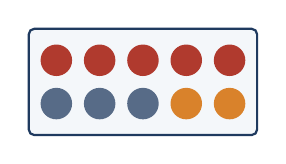
\begin{tikzpicture}
\draw[navy,thick,fill=softbg,rounded corners=2pt] (0,0) rectangle (2.9,1.35);
\foreach \k in {0,...,4}{\fill[brick] (0.35+0.55*\k,0.95) circle (0.2);}
\foreach \k in {0,...,2}{\fill[navy!75] (0.35+0.55*\k,0.4) circle (0.2);}
\foreach \k in {3,4}{\fill[amber] (0.35+0.55*\k,0.4) circle (0.2);}
\end{tikzpicture}}}{\begin{tabularx}{\linewidth}{@{}*{5}{X}@{}}\textbf{A.}\;$\dis\frac18$ & \textbf{B.}\;$\dis\frac16$ & \textbf{C.}\;$\dis\frac14$ & \textbf{D.}\;$\dis\frac3{10}$ & \textbf{E.}\;$\dis\frac13$\end{tabularx}}
\soal{\gbr{Sebuah kotak berisi $5$ bola merah dan $3$ bola putih. Dua bola diambil satu per satu tanpa pengembalian. Diagram pohon pada gambar menunjukkan peluang tiap pengambilan ($M$ = merah, $P$ = putih). Peluang kedua bola berbeda warna adalah \dots.}{%
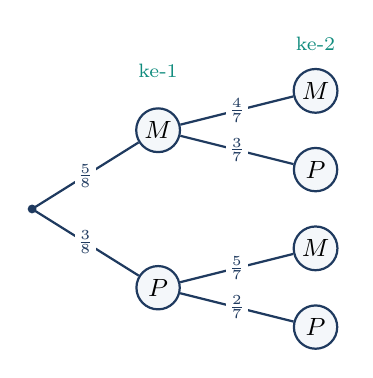
\begin{tikzpicture}
\coordinate (O) at (0,0);
\node[nd] (M) at (1.6,1.0) {$M$}; \node[nd] (P) at (1.6,-1.0) {$P$};
\node[nd] (MM) at (3.6,1.5) {$M$}; \node[nd] (MP) at (3.6,0.5) {$P$};
\node[nd] (PM) at (3.6,-0.5) {$M$}; \node[nd] (PP) at (3.6,-1.5) {$P$};
\fill[navy] (O) circle (1.6pt);
\draw[navy,thick] (O)--(M) node[lf]{$\frac58$};
\draw[navy,thick] (O)--(P) node[lf]{$\frac38$};
\draw[navy,thick] (M)--(MM) node[lf]{$\frac47$};
\draw[navy,thick] (M)--(MP) node[lf]{$\frac37$};
\draw[navy,thick] (P)--(PM) node[lf]{$\frac57$};
\draw[navy,thick] (P)--(PP) node[lf]{$\frac27$};
\node[font=\scriptsize,teal] at (1.6,1.75) {ke-1}; \node[font=\scriptsize,teal] at (3.6,2.1) {ke-2};
\end{tikzpicture}}}{\begin{tabularx}{\linewidth}{@{}*{5}{X}@{}}\textbf{A.}\;$\dis\frac3{14}$ & \textbf{B.}\;$\dis\frac5{14}$ & \textbf{C.}\;$\dis\frac12$ & \textbf{D.}\;$\dis\frac{15}{28}$ & \textbf{E.}\;$\dis\frac9{14}$\end{tabularx}}
\soal{\gbr{Diagram Venn pada gambar menunjukkan persentase siswa suatu sekolah yang menyukai matematika ($M$) dan fisika ($F$). Seorang siswa dipilih secara acak. Jika diketahui siswa itu menyukai matematika, peluang ia juga menyukai fisika adalah \dots.}{%
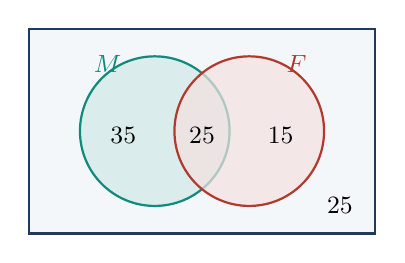
\begin{tikzpicture}
\draw[navy,thick,fill=softbg] (-2.2,-1.3) rectangle (2.2,1.3);
\draw[teal,thick,fill=teal!20,fill opacity=0.7] (-0.6,0) circle (0.95);
\draw[brick,thick,fill=brick!15,fill opacity=0.7] (0.6,0) circle (0.95);
\node[teal,font=\small\bfseries] at (-1.2,0.85) {$M$}; \node[brick,font=\small\bfseries] at (1.2,0.85) {$F$};
\node[font=\small] at (-1.0,-0.05) {$35$}; \node[font=\small] at (0,-0.05) {$25$}; \node[font=\small] at (1.0,-0.05) {$15$};
\node[font=\small] at (1.75,-0.95) {$25$};
\end{tikzpicture}}}{\begin{tabularx}{\linewidth}{@{}*{5}{X}@{}}\textbf{A.}\;$\dis\frac14$ & \textbf{B.}\;$\dis\frac13$ & \textbf{C.}\;$\dis\frac5{12}$ & \textbf{D.}\;$\dis\frac12$ & \textbf{E.}\;$\dis\frac58$\end{tabularx}}
\soal{Kejadian $A$ dan $B$ saling bebas dengan $P(A)=0{,}4$ dan $P(A\cup B)=0{,}7$. Nilai $P(B)$ adalah \dots.}{\begin{tabularx}{\linewidth}{@{}*{5}{X}@{}}\textbf{A.}\;$0{,}30$ & \textbf{B.}\;$0{,}35$ & \textbf{C.}\;$0{,}40$ & \textbf{D.}\;$0{,}45$ & \textbf{E.}\;$0{,}50$\end{tabularx}}
\soal{Sebuah dadu seimbang dilempar $4$ kali. Peluang muncul mata $6$ tepat dua kali adalah \dots.}{\begin{tabularx}{\linewidth}{@{}*{5}{X}@{}}\textbf{A.}\;$\dis\frac{25}{216}$ & \textbf{B.}\;$\dis\frac5{36}$ & \textbf{C.}\;$\dis\frac{25}{108}$ & \textbf{D.}\;$\dis\frac{25}{72}$ & \textbf{E.}\;$\dis\frac{125}{216}$\end{tabularx}}

\tingkat{Tingkat Sulit}{soal 11 sampai 15, setara UTBK}
\soal{Suatu penyakit diderita oleh $10\%$ penduduk sebuah kota. Alat tes menunjukkan hasil positif pada $90\%$ penderita, tetapi juga positif pada $5\%$ orang yang tidak sakit. Seseorang dipilih acak dan hasil tesnya positif. Peluang ia benar-benar sakit adalah \dots.}{\begin{tabularx}{\linewidth}{@{}*{5}{X}@{}}\textbf{A.}\;$\dis\frac15$ & \textbf{B.}\;$\dis\frac13$ & \textbf{C.}\;$\dis\frac12$ & \textbf{D.}\;$\dis\frac35$ & \textbf{E.}\;$\dis\frac23$\end{tabularx}}
\soal{\gbr{Enam orang, termasuk $A$, $B$, dan $C$, duduk mengelilingi sebuah meja bundar dengan enam kursi (lihat gambar). Jika susunan duduk dilakukan secara acak, peluang $A$, $B$, dan $C$ duduk berdampingan (berurutan, urutan di antara mereka bebas) adalah \dots.}{%
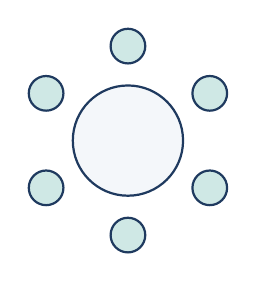
\begin{tikzpicture}
\draw[navy,thick,fill=softbg] (0,0) circle (0.7);
\foreach \i in {0,...,5}{\draw[navy,thick,fill=teal!20] ({90+60*\i}:1.2) circle (0.22);}
\end{tikzpicture}}}{\begin{tabularx}{\linewidth}{@{}*{5}{X}@{}}\textbf{A.}\;$\dis\frac15$ & \textbf{B.}\;$\dis\frac3{10}$ & \textbf{C.}\;$\dis\frac25$ & \textbf{D.}\;$\dis\frac12$ & \textbf{E.}\;$\dis\frac35$\end{tabularx}}
\soal{Dua dadu seimbang dilempar bersamaan. Nilai harapan selisih mutlak kedua mata dadu adalah \dots.}{\begin{tabularx}{\linewidth}{@{}*{5}{X}@{}}\textbf{A.}\;$\dis\frac53$ & \textbf{B.}\;$\dis\frac74$ & \textbf{C.}\;$\dis\frac{35}{18}$ & \textbf{D.}\;$2$ & \textbf{E.}\;$\dis\frac73$\end{tabularx}}
\soal{Tiga bilangan berbeda dipilih secara acak dari himpunan $\{1,2,\dots,9\}$. Peluang jumlah ketiga bilangan itu ganjil adalah \dots.}{\begin{tabularx}{\linewidth}{@{}*{5}{X}@{}}\textbf{A.}\;$\dis\frac{10}{21}$ & \textbf{B.}\;$\dis\frac12$ & \textbf{C.}\;$\dis\frac{11}{21}$ & \textbf{D.}\;$\dis\frac59$ & \textbf{E.}\;$\dis\frac47$\end{tabularx}}
\soal{Dua dadu seimbang dilempar bersamaan. Jika diketahui jumlah kedua mata dadu tidak lebih dari $7$, peluang paling sedikit satu dadu menunjukkan mata $5$ adalah \dots.}{\begin{tabularx}{\linewidth}{@{}*{5}{X}@{}}\textbf{A.}\;$\dis\frac17$ & \textbf{B.}\;$\dis\frac4{21}$ & \textbf{C.}\;$\dis\frac27$ & \textbf{D.}\;$\dis\frac5{21}$ & \textbf{E.}\;$\dis\frac13$\end{tabularx}}

\bagian{B. Isian Singkat}{5 soal $\times$ 5 poin = 25 poin. Tuliskan hanya jawaban akhir.}
\soal{Dua dadu seimbang dilempar bersamaan. Peluang jumlah kedua mata dadu berupa bilangan prima adalah \dots}{\hfill Jawaban: \rule{4.5cm}{0.4pt}}
\soal{Sebuah panitia beranggotakan $4$ orang dipilih secara acak dari $6$ pria dan $4$ wanita. Peluang panitia itu terdiri atas $2$ pria dan $2$ wanita adalah \dots}{\hfill Jawaban: \rule{4.5cm}{0.4pt}}
\soal{Variabel acak $X$ berdistribusi binomial dengan $E(X)=6$ dan $\operatorname{Var}(X)=4{,}2$. Nilai $n$ adalah \dots}{\hfill Jawaban: \rule{4.5cm}{0.4pt}}
\soal{\gbr{Papan sasaran berbentuk tiga lingkaran sepusat dengan jari-jari $2$ cm, $4$ cm, dan $6$ cm (lihat gambar). Sebuah anak panah mengenai papan secara acak. Peluang anak panah mengenai daerah yang diwarnai (di antara lingkaran berjari-jari $2$ cm dan $4$ cm) adalah \dots}{%
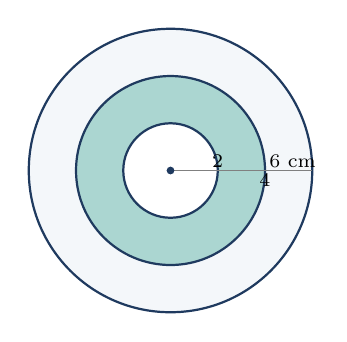
\begin{tikzpicture}
\fill[softbg] (0,0) circle (1.8);
\fill[teal!35] (0,0) circle (1.2);
\fill[white] (0,0) circle (0.6);
\draw[navy,thick] (0,0) circle (0.6); \draw[navy,thick] (0,0) circle (1.2); \draw[navy,thick] (0,0) circle (1.8);
\draw[gray] (0,0)--(1.8,0);
\fill[navy] (0,0) circle (1.4pt);
\node[above,font=\scriptsize,inner sep=1pt] at (0.6,0) {$2$}; \node[below,font=\scriptsize,inner sep=1pt] at (1.2,0) {$4$}; \node[above,font=\scriptsize,inner sep=1pt] at (1.55,0) {$6$ cm};
\end{tikzpicture}}}{\hfill Jawaban: \rule{4.5cm}{0.4pt}}
\soal{Seorang pemanah mengenai sasaran dengan peluang $0{,}6$ pada setiap tembakan, dan tembakan-tembakan itu saling bebas. Banyak tembakan minimum agar peluang mengenai sasaran sedikitnya satu kali lebih dari $0{,}99$ adalah \dots}{\hfill Jawaban: \rule{4.5cm}{0.4pt}}

\bagian{C. Uraian (Essay)}{3 soal $\times$ 10 poin = 30 poin. Tuliskan langkah penyelesaian dengan lengkap.}
\soal{\gbr{Kotak I berisi $4$ bola merah dan $3$ bola putih, sedangkan kotak II berisi $2$ bola merah dan $5$ bola putih (lihat gambar). Sebuah koin seimbang dilempar: jika muncul gambar, diambil satu bola dari kotak I; jika muncul angka, diambil satu bola dari kotak II.\par\smallskip(a) Tentukan peluang bola yang terambil berwarna merah.\par(b) Jika bola yang terambil berwarna putih, tentukan peluang bola itu berasal dari kotak I.\par(c) Dua bola diambil sekaligus dari kotak I. Tentukan peluang keduanya sewarna.\par(d) Dua bola diambil satu per satu tanpa pengembalian dari kotak II. Tentukan peluang keduanya putih.}{%
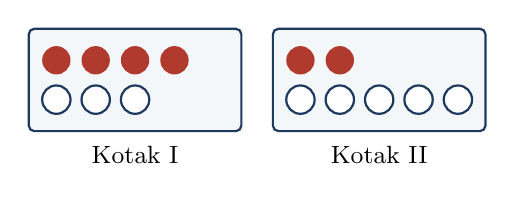
\begin{tikzpicture}
\draw[navy,thick,fill=softbg,rounded corners=2pt] (0,0) rectangle (2.7,1.3);
\foreach \k in {0,...,3}{\fill[brick] (0.35+0.5*\k,0.9) circle (0.18);}
\foreach \k in {0,...,2}{\draw[navy,thick,fill=white] (0.35+0.5*\k,0.4) circle (0.18);}
\node[font=\small] at (1.35,-0.3) {Kotak I};
\begin{scope}[xshift=3.1cm]
\draw[navy,thick,fill=softbg,rounded corners=2pt] (0,0) rectangle (2.7,1.3);
\foreach \k in {0,1}{\fill[brick] (0.35+0.5*\k,0.9) circle (0.18);}
\foreach \k in {0,...,4}{\draw[navy,thick,fill=white] (0.35+0.5*\k,0.4) circle (0.18);}
\node[font=\small] at (1.35,-0.3) {Kotak II};
\end{scope}
\end{tikzpicture}}}{\poin{10}}
\soal{\gbr{Dua dadu seimbang dilempar bersamaan. Misalkan $A$ adalah kejadian jumlah kedua mata dadu sama dengan $8$ dan $B$ adalah kejadian kedua mata dadu genap. Pada gambar, ke-$36$ hasil yang mungkin ditunjukkan sebagai titik, titik hijau menandai kejadian $B$, dan lingkaran merah menandai kejadian $A$.\par\smallskip(a) Tentukan $n(S)$, $n(A)$, dan $n(B)$.\par(b) Tentukan $P(A\cup B)$.\par(c) Tentukan $P(B\mid A)$.\par(d) Apakah $A$ dan $B$ saling bebas? Jelaskan.}{%
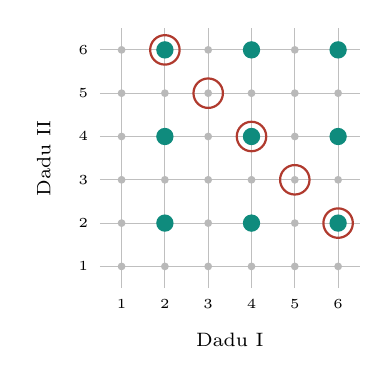
\begin{tikzpicture}[scale=0.55]
\draw[gray!50,thin] (0.5,0.5) grid (6.5,6.5);
\foreach \a in {1,...,6}{\foreach \b in {1,...,6}{%
  \pgfmathtruncatemacro{\s}{\a+\b}
  \fill[gray!55] (\a,\b) circle (0.09);
  \ifodd\a\else\ifodd\b\else\fill[teal] (\a,\b) circle (0.2);\fi\fi
  \ifnum\s=8 \draw[brick,thick] (\a,\b) circle (0.34);\fi}}
\foreach \i in {1,...,6}{\node[font=\tiny,below] at (\i,0.45) {\i}; \node[font=\tiny,left] at (0.45,\i) {\i};}
\node[font=\scriptsize] at (3.5,-0.7) {Dadu I}; \node[font=\scriptsize,rotate=90] at (-0.8,3.5) {Dadu II};
\end{tikzpicture}}}{\poin{10}}
\soal{(a) Buktikan bahwa jika kejadian $A$ dan $B$ saling bebas, maka $A$ dan $B^{c}$ juga saling bebas.\par\smallskip(b) Dua penembak, $A$ dan $B$, menembak sasaran secara serentak dan saling bebas. Peluang $A$ mengenai sasaran adalah $0{,}8$ dan peluang $B$ mengenai sasaran adalah $0{,}7$. Tentukan peluang bahwa (i) tepat satu penembak mengenai sasaran, dan (ii) sedikitnya satu penembak mengenai sasaran.\par(c) Jika $B$ menembak $4$ kali secara bebas, tentukan peluang $B$ mengenai sasaran tepat $3$ kali.}{\poin{10}}

\newpage
\bagian{Kunci Jawaban dan Pembahasan Singkat}{Untuk guru dan pembahasan mandiri}
\par\vspace{0.6em}{\bfseries\color{navy}Kunci Pilihan Ganda}\par\vspace{0.3em}
\small
\begin{tabularx}{\linewidth}{@{}*{15}{>{\centering\arraybackslash}X}@{}}\hline \textbf{1} & \textbf{2} & \textbf{3} & \textbf{4} & \textbf{5} & \textbf{6} & \textbf{7} & \textbf{8} & \textbf{9} & \textbf{10} & \textbf{11} & \textbf{12} & \textbf{13} & \textbf{14} & \textbf{15}\\ \hline C & A & D & B & E & C & D & C & E & A & E & B & C & A & B\\ \hline\end{tabularx}
\par\vspace{0.8em}{\bfseries\color{navy}\normalsize Pembahasan Pilihan Ganda}\par\vspace{0.2em}
\small\begin{enumerate}[leftmargin=2em,itemsep=2pt,topsep=2pt]
\item[\textbf{1.}] \textbf{(C)} Ada $10$ sektor sama besar. Bilangan prima: $2,3,5,7$ (ada $4$ sektor). Maka $P=\dis\frac4{10}=\dis\frac25$.
\item[\textbf{2.}] \textbf{(A)} Jumlah $9$: $4$ cara, jumlah $10$: $3$ cara, jumlah $11$: $2$ cara, jumlah $12$: $1$ cara, totalnya $10$ cara. Maka $P=\dis\frac{10}{36}=\dis\frac5{18}$.
\item[\textbf{3.}] \textbf{(D)} Kelipatan $3$: $3,6,9,12$ (4 kartu). Kelipatan $4$: $4,8,12$ (3 kartu). Irisan: $12$ (1 kartu). Maka $n(A\cup B)=4+3-1=6$ dan $P=\dis\frac6{12}=\dis\frac12$.
\item[\textbf{4.}] \textbf{(B)} Banyak percobaan $=6+8+9+7+12+8=50$. Frekuensi mata genap ($2,4,6$) $=8+7+8=23$. Peluang empirisnya $\dis\frac{23}{50}$.
\item[\textbf{5.}] \textbf{(E)} Peluang tidak rusak $=1-0{,}04=0{,}96$. Frekuensi harapan $=500\times0{,}96=480$.
\item[\textbf{6.}] \textbf{(C)} Dari gambar: $5$ merah, $3$ biru, $2$ kuning. $n(S)=\dbinom{10}{3}=120$ dan $n(A)=5\cdot3\cdot2=30$. Maka $P=\dis\frac{30}{120}=\dis\frac14$.
\item[\textbf{7.}] \textbf{(D)} Berbeda warna: $MP$ atau $PM$. $P=\dis\frac58\cdot\dis\frac37+\dis\frac38\cdot\dis\frac57=\dis\frac{15}{56}+\dis\frac{15}{56}=\dis\frac{30}{56}=\dis\frac{15}{28}$.
\item[\textbf{8.}] \textbf{(C)} Yang menyukai matematika: $35+25=60$. Yang menyukai matematika dan fisika: $25$. Maka $P(F\mid M)=\dis\frac{25}{60}=\dis\frac5{12}$.
\item[\textbf{9.}] \textbf{(E)} Karena saling bebas, $P(A\cup B)=P(A)+P(B)-P(A)P(B)$. Jadi $0{,}7=0{,}4+P(B)-0{,}4\,P(B)=0{,}4+0{,}6\,P(B)$, sehingga $P(B)=\dis\frac{0{,}3}{0{,}6}=0{,}5$.
\item[\textbf{10.}] \textbf{(A)} $P=\dbinom42\left(\dis\frac16\right)^{2}\left(\dis\frac56\right)^{2}=6\cdot\dis\frac{25}{1296}=\dis\frac{150}{1296}=\dis\frac{25}{216}$.
\item[\textbf{11.}] \textbf{(E)} Misalkan $S$ = sakit dan $T$ = tes positif. $P(T)=0{,}1\cdot0{,}9+0{,}9\cdot0{,}05=0{,}09+0{,}045=0{,}135$. Dengan Bayes, $P(S\mid T)=\dis\frac{0{,}09}{0{,}135}=\dis\frac23$.
\item[\textbf{12.}] \textbf{(B)} Susunan melingkar $6$ orang: $(6-1)!=120$. Anggap $A,B,C$ satu kelompok: ada $(4-1)!=6$ susunan, dan di dalam kelompok ada $3!=6$ susunan. Maka $P=\dis\frac{6\cdot6}{120}=\dis\frac{36}{120}=\dis\frac3{10}$.
\item[\textbf{13.}] \textbf{(C)} Banyak pasangan dengan selisih $0,1,2,3,4,5$ berturut-turut adalah $6,10,8,6,4,2$. Jumlah selisih $\times$ banyak pasangan $=0\cdot6+1\cdot10+2\cdot8+3\cdot6+4\cdot4+5\cdot2=70$, sehingga $E=\dis\frac{70}{36}=\dis\frac{35}{18}$.
\item[\textbf{14.}] \textbf{(A)} Jumlah ganjil terjadi bila banyak bilangan ganjil yang terpilih ganjil. Ada $5$ bilangan ganjil dan $4$ genap. Satu ganjil dan dua genap: $5\cdot\dbinom42=30$. Tiga ganjil: $\dbinom53=10$. Maka $P=\dis\frac{40}{\dbinom93}=\dis\frac{40}{84}=\dis\frac{10}{21}$.
\item[\textbf{15.}] \textbf{(B)} Jumlah $\le7$: $1+2+3+4+5+6=21$ hasil. Di antaranya yang memuat mata $5$: $(5,1),(5,2),(1,5),(2,5)$, yaitu $4$ hasil. Maka $P=\dis\frac4{21}$.
\end{enumerate}
\par\Needspace{6\baselineskip}\vspace{0.6em}{\bfseries\color{navy}\normalsize Pembahasan Isian Singkat}\par\vspace{0.2em}
\small\begin{enumerate}[leftmargin=2em,itemsep=2pt,topsep=2pt]
\item[\textbf{1.}] \textbf{Jawaban: $\dis\frac5{12}$.} Jumlah prima: $2$ (1 cara), $3$ (2 cara), $5$ (4 cara), $7$ (6 cara), $11$ (2 cara), totalnya $15$ cara. $P=\dis\frac{15}{36}=\dis\frac5{12}$.
\item[\textbf{2.}] \textbf{Jawaban: $\dis\frac37$.} $P=\dis\frac{\dbinom62\dbinom42}{\dbinom{10}4}=\dis\frac{15\cdot6}{210}=\dis\frac{90}{210}=\dis\frac37$.
\item[\textbf{3.}] \textbf{Jawaban: $20$.} $np=6$ dan $np(1-p)=4{,}2$, sehingga $1-p=\dis\frac{4{,}2}{6}=0{,}7$ dan $p=0{,}3$. Maka $n=\dis\frac{6}{0{,}3}=20$.
\item[\textbf{4.}] \textbf{Jawaban: $\dis\frac13$.} Luas papan $=\pi\cdot6^{2}=36\pi$. Luas daerah yang diwarnai $=\pi(4^{2}-2^{2})=12\pi$. Maka $P=\dis\frac{12\pi}{36\pi}=\dis\frac13$.
\item[\textbf{5.}] \textbf{Jawaban: $6$.} Peluang sedikitnya satu kali mengenai $=1-(0{,}4)^{n}>0{,}99$, yaitu $(0{,}4)^{n}<0{,}01$. Karena $(0{,}4)^{5}=0{,}01024>0{,}01$ dan $(0{,}4)^{6}=0{,}004096<0{,}01$, maka $n$ minimum $=6$.
\end{enumerate}
\par\Needspace{8\baselineskip}\vspace{0.6em}{\bfseries\color{navy}\normalsize Pembahasan dan Pedoman Penskoran Uraian}\par\vspace{0.2em}
\small\begin{enumerate}[leftmargin=2em,itemsep=3pt,topsep=2pt]
\item[\textbf{1.}] (a) $P(M)=P(\text{I})P(M\mid\text{I})+P(\text{II})P(M\mid\text{II})=\dis\frac12\cdot\dis\frac47+\dis\frac12\cdot\dis\frac27=\dis\frac27+\dis\frac17=\dis\frac37$. (b) $P(\text{putih})=1-\dis\frac37=\dis\frac47$ dan $P(\text{I}\cap\text{putih})=\dis\frac12\cdot\dis\frac37=\dis\frac3{14}$. Maka $P(\text{I}\mid\text{putih})=\dis\frac{3/14}{4/7}=\dis\frac38$. (c) $n(S)=\dbinom72=21$. Sewarna: $\dbinom42+\dbinom32=6+3=9$. Maka $P=\dis\frac9{21}=\dis\frac37$. (d) $P=\dis\frac57\cdot\dis\frac46=\dis\frac{20}{42}=\dis\frac{10}{21}$. \\ \textit{Penskoran: (a) 3 poin; (b) 3 poin; (c) 2 poin; (d) 2 poin.}
\item[\textbf{2.}] (a) $n(S)=36$. $A=\{(2,6),(3,5),(4,4),(5,3),(6,2)\}$, sehingga $n(A)=5$. Kedua mata genap, masing-masing dari $\{2,4,6\}$, sehingga $n(B)=3\cdot3=9$. (b) $A\cap B=\{(2,6),(4,4),(6,2)\}$, sehingga $n(A\cap B)=3$. Maka $n(A\cup B)=5+9-3=11$ dan $P(A\cup B)=\dis\frac{11}{36}$. (c) $P(B\mid A)=\dis\frac{n(A\cap B)}{n(A)}=\dis\frac35$. (d) $P(B)=\dis\frac9{36}=\dis\frac14\neq\dis\frac35=P(B\mid A)$. (Atau: $P(A\cap B)=\dis\frac3{36}=\dis\frac{12}{144}$, sedangkan $P(A)P(B)=\dis\frac5{36}\cdot\dis\frac14=\dis\frac5{144}$.) Karena tidak sama, $A$ dan $B$ tidak saling bebas. \\ \textit{Penskoran: (a) 3 poin (masing-masing 1 poin); (b) 3 poin; (c) 2 poin; (d) 2 poin.}
\item[\textbf{3.}] (a) Karena $A=(A\cap B)\cup(A\cap B^{c})$ dengan kedua bagian saling lepas, maka $P(A\cap B^{c})=P(A)-P(A\cap B)$. Karena $A$ dan $B$ saling bebas, $P(A\cap B)=P(A)P(B)$, sehingga $P(A\cap B^{c})=P(A)-P(A)P(B)=P(A)\left[1-P(B)\right]=P(A)P(B^{c})$. Jadi $A$ dan $B^{c}$ saling bebas. (b) (i) Tepat satu mengenai: $0{,}8\cdot0{,}3+0{,}2\cdot0{,}7=0{,}24+0{,}14=0{,}38$. (ii) Sedikitnya satu mengenai: $1-P(\text{keduanya meleset})=1-0{,}2\cdot0{,}3=1-0{,}06=0{,}94$. (c) $P=\dbinom43(0{,}7)^{3}(0{,}3)=4\cdot0{,}343\cdot0{,}3=0{,}4116$. \\ \textit{Penskoran: (a) 3 poin; (b) 4 poin (masing-masing 2 poin); (c) 3 poin (rumus binomial 2 poin, hasil 1 poin).}
\end{enumerate}
\end{document}
